%%%%%%%%%%%%%%%%%%%%%%% file template.tex %%%%%%%%%%%%%%%%%%%%%%%%%
%
% This is a general template file for the LaTeX package SVJour3
% for Springer journals.          Springer Heidelberg 2006/03/15
%
% Copy it to a new file with a new name and use it as the basis
% for your article. Delete % signs as needed.
%
% This template includes a few options for different layouts and
% content for various journals. Please consult a previous issue of
% your journal as needed.
%
%%%%%%%%%%%%%%%%%%%%%%%%%%%%%%%%%%%%%%%%%%%%%%%%%%%%%%%%%%%%%%%%%%%
%
% First comes an example EPS file -- just ignore it and
% proceed on the \documentclass line
% your LaTeX will extract the file if required
\begin{filecontents*}{example.eps}
%!PS-Adobe-3.0 EPSF-3.0
%%BoundingBox: 19 19 221 221
%%CreationDate: Mon Sep 29 1997
%%Creator: programmed by hand (JK)
%%EndComments
gsave
newpath
  20 20 moveto
  20 220 lineto
  220 220 lineto
  220 20 lineto
closepath
2 setlinewidth
gsave
  .4 setgray fill
grestore
stroke
grestore
\end{filecontents*}
%
\documentclass{svjour3}                     % onecolumn (standard format)
%\documentclass[smallextended]{svjour3}     % onecolumn (second format)
%\documentclass[twocolumn]{svjour3}         % twocolumn
%
\smartqed  % flush right qed marks, e.g. at end of proof
%
\usepackage{graphicx}
%
% \usepackage{mathptmx}      % use Times fonts if available on your TeX system
%
% insert here the call for the packages your document requires
%\usepackage{latexsym}
% etc.
%
% please place your own definitions here and don't use \def but
% \newcommand{}{}
%
% Insert the name of "your journal" with
\journalname{JournalofGridComputing}
%
\begin{document}

\title{Distributed Analysis in CMS}
%\subtitle{Do you have a subtitle?\\ If so, write it here}

\author{Alessandra Fanfani \and Andrea Sciab`a \and Anzar Afaq \and Carlos Kavka \and Chih-Hao Huang \and Christoph Wissing \and Claudio Grandi \and Daniele Bonacorsi \and Daniele Spiga \and Daniel Riley \and Dave Evans \and Eric Vaandering \and Fabio Farina \and Federica Fanzago \and Frank Wuerthwein \and Giuseppe Codispoti \and Hassen Riahi \and Ian Fisk \and Ilaria Villella \and James Letts \and Jorgen D'Hondt \and Joris Maes \and Jose' M. Hern´andez \and Joseph Flix \and Jukka Klem \and Julia Andreeva \and Marco Calloni \and Mattia Cinquilli \and Niccolo' Magini \and Pablo Saiz \and Petra Van Mulders \and Ricky Egeland \and Sanjay Padhi \and Simon Metson  \and Stefano Belforte \and Stefano Lacaprara \and Thomas Kress \and Tony Wildish \and Valentin Kuznetsov \and Vijay Sekhri \and Vincenzo Miccio \and Yuyi Guo }

\authorrunning{ Alessandra Fanfani \and Andrea Sciab`a \and Anzar Afaq \and Carlos Kavka \and Chih-Hao Huang \and Chris Brew \and Christoph Wissing \and Claudio Grandi \and Daniele Bonacorsi \and Daniele Spiga \and Daniel Riley \and Dave Evans \and David Colling \and Eric Vaandering \and Fabio Farina \and Federica Fanzago \and Frank Wuerthwein \and Gerhild Maier \and Giuseppe Bagliesi \and Giuseppe Codispoti \and Hassen Riahi \and Ian Fisk \and Ilaria Villella \and James Letts \and Jorgen D'Hondt \and Joris Maes \and Jose' M. Hern´andez \and Joseph Flix \and Jukka Klem \and Julia Andreeva \and Ken Bloom \and Marco Calloni \and Mattia Cinquilli \and Niccolo' Magini \and Pablo Saiz \and Peter Kreuzer \and Petra Van Mulders \and Ricky Egeland \and Sanjay Padhi \and Simon Metson  \and Stefano Belforte \and Stefano Lacaprara \and Subir Sarkar \and Thomas Kress \and Tony Wildish \and Valentin Kuznetsov \and Vijay Sekhri \and Vincenzo Miccio \and Yuyi Guo} % if too long for running head

\institute{A. Fanfani \and D. Bonacorsi \and G. Codispoti \and C. Grandi
           \at INFN and University of Bologna, viale Berti Pichat 6/2, 40127 Bologna, Italy \\
              Tel.: +39-51-2095232 Fax: +39-51-209XXXX\\
              \email{fanfani@bo.infn.it}
%             \emph{Present address:} of F. Author  %  if needed
           \and 
            M. Calloni \and N. Magini \and D. Spiga \and J. Andreeva \and P. Saiz \and V. Miccio \at CERN, Switzerland
           \and
           S. Lacaprara \at Legnaro INFN, Italy
           \and
           F. Fanzago \at Padova INFN, Italy
           \and 
           S. Belforte \and C. Kavka \at Trieste INFN, Italy
           \and
           F. Farina \at Milano Bicocca INFN, Italy
           \and
           M. Cinquilli \and H. Riahi \at Perugia INFN, Italy
           \and
           S. Metson \at Bristol University, UK
           \and
           C. Wissing \at DESY,  Germany
           T. Kress \at RWTH , Germany
           \and
           J. D'Hondt \and J.Maes \and P. Van Mulders \and I. Villella \at Brussel University, Belgium
           \and
           J. Klem \at Helsinki Institute of Physics, Finland
           \and
            J. M. Hern´andez \at CIEMAT, Madrid, Spain
           \and
            J. Flix \at PIC, Barcelona, Spain
           \and
           A. Afaq \and D. Evans \and I. Fisk \and Y. Guo \and C. Huang \and V. Sekhri \and E.Vaandering \at Fermilab, Batavia, Illinois, USA
           \and 
           V. Kuznetsov \and D. Riley \at Cornell University, Ithaca, New York, USA 
           \and 
           R. Egeland \at Minnesota University, Twin Cities, USA
           \and 
           T. Wildish \at Princeton University, USA
           \and
           J. Letts \and S. Padhi \and F. Wuerthwein \at S. Diego University, USA
}

\date{Received: date / Accepted: date}
% The correct dates will be entered by the editor


\maketitle

\begin{abstract}
Bla bla bla bla bla bla bla bla bla bla bla bla bla bla bla bla bla bla bla bla bla bla bla bla bla bla bla bla bla bla bla bla bla bla bla bla bla bla bla bla bla bla bla bla blabla bla bla bla bla bla bla bla bla bla bla bla bla bla bla bla bla bla bla bla bla bla bla bla bla bla bla bla bla bla bla bla bla bla bla bla bla bla bla bla bla bla bla bla bla bla bla bla bla bla bla bla bla bla bla bla bla bla bla blabla bla bla bla bla bla bla bla bla bla bla bla bla bla bla bla bla bla bla bla bla bla bla bla bla bla bla bla bla bla bla bla bla bla bla bla bla bla blabla bla bla bla bla bla bla bla bla bla bla bla bla bla bla bla bla bla bla bla bla bla bla bla bla bla bla bla bla bla bla bla bla bla bla bla
\keywords{LHC \and CMS \and Distributed Analysis}
% \PACS{PACS code1 \and PACS code2 \and more}
% \subclass{MSC code1 \and MSC code2 \and more}
\end{abstract}

\section{Introduction}
\label{intro}
\emph{Bla bla bla bla bla CMS\cite{RefCMS}.
A large experimental community, more
than 3000 collaborators, distributed over more than 38 countries all around the world ..... bla bla bla}

%\paragraph{Paragraph headings} Use paragraph headings as needed.
\section{The CMS Computing Model}
\label{sec:2}
The CMS distributed computing and analysis model is designed to serve, process and archive the %huge amount of data the experiment will collect.
%large amounts of events that will be available when the detector starts collecting data.
large number of events that will be generated when the CMS detector starts taking data. The computing resources are geographically distributed, interconnected via high throughput networks and operated by means of Grid software. 
%%  motivations to choose a distributed environment
The choice of a distributed system allows to delegate responsibilities to local CMS communities, access to additional funding channels and ensure load balancing of the available resources while replicating the interesting data in different sites.


A multi-Tier hierarchical distributed model is adopted in CMS with specific functionality at different levels.
\subsection{Tier-0}
\label{sec:2_1}
The Tier-0 centre at CERN accepts data from the CMS online system, archives the data, performs prompt first pass reconstruction. Reconstructed data at the Tier-0 together with the corresponding raw data are distributed to Tier-1s over the optical private network. In addition to the Tier-0 centre, CERN hosts the CMS Analysis Facility (CAF) that is focused on latency-critical detector, trigger and calibration activities.
Roughly 20\% of the computing capacity is located at CERN, while the remaining is distributed.

\subsection{Tier-1}
\label{sec:2_2}
Each Tier-1 centre assures the distributed custodial storage of a fraction of the RAW data produced by the CMS detector and for the simulated data produced at the connected Tier-2 centres; provides computing resources for their further re-processing (re-reconstruction, skimming, etc…) and for high priority analysis; controls the data transfer to the Tier-2 centres for analysis. There are 7 Tier-1 centres located in France, Germany, Italy, Spain, Taiwan, United Kingdom and United States.

%The Tier-1 are 7 large regional computing centers located in France, Germany, Italy, Spain, Taiwan, United Kingdom and United States, where organized mass data processing are performed. That includes re-processing, data skimming and other organized intensive analysis tasks. 
%%From CM CHEP09: For reconstruction a nominal Tier-1 should be capable of processing 70Hz worth of data with a required IO rate of 100MB/s. Skimming through the reconstructed datasets uses only 1\% of CPU of reconstruction so sparse reading of the file is required to have manageable IO rates.
%The Tier-1 centres archive the fraction of data distributed to them as well as the simulated data produced at the Tier-2 centres,  while they are serving analysis transfer requests to Tier-2.
%%From CM CHEP09: In the CMS experiment the Tier-1 centers rather than the Tier-0 serve the majority of the data to the Tier-2 centers for analysis.

\subsection{Tier-2}
\label{sec:2_3}
Tier-2 centers provide capacity for user data analysis and for production of simulated data.
In CMS data transfer to Tier-2 can occur from any Tier-1. A significant effort is required in 
commissioning all possible transfer links, as described in section ~\ref{sec:4_1_4}, as well
as improving site availability, as described in section ~\ref{sec:4_1_3}.

\section{Framework for CMS Distributed Analysis}
\label{sec:3}
The CMS analysis model foresees activites driven by data location. Data are scattered over many computing centers according to CMS data placement policies and processing takes place where data are located. In order to enable distributed analysis a set of Workload and Data Management tools have been designed, building CMS-specific services on top of existing Grid ones.

\subsection{Data Management}
\label{sec:3_1}
The CMS Data Management System provides the basic infrastructure and tools necessary to manage the large amounts of data produced, processed and analysed in a distributed computing environment. 
In order to simplify bulk data management, files are grouped together into “file-blocks”  of a convenient size for data transfer. %the exact choice of the size of the file blocks will depend on the type of data. 
File-blocks are in turn grouped in datasets whose size is driven by physics.
The file-block is the unit of data location and replication. 
The tracking of data location is file-block based and it provides the name of sites hosting the data, not the physical location of constituent files at the sites nor the composition of file-blocks.
The file-block contains files that can be processed and analyzed together.
%Processing is block-based. 
The packaging of events into files is done so that the average file size is
kept reasonably large (e.g. at least 1GB), in order to avoid scaling issues with storage and tape systems and to optimize data transfer.
This is achieved merging small outputs files produced by individual jobs in fewer larger files.

The CMS Data Management System is made of a set of loosely coupled components as described in the following sections.
\subsubsection{DBS}
\label{sec:3_1_1}
The Dataset Bookkeeping Service (DBS)\cite{RefDBS} provides the means to describe, discover and use CMS event data. 
It catalogs CMS specific data definitions such as run number, the algorithms and configurations used to process the data toghether with the information regarding the processing parentage of the data it describes.
The DBS stores information about CMS data in a queryable format. The supported queries allow to discover available data and how they are organized logically in term of packaging units like files and file-blocks. The information available from queries to DBS are site independent.

The DBS is used for data discovery and job configuration by the production and analysis systems through a DBS API. 
Users can discover what data exists using a Web browser or Command Line Interface.
The DBS is usable in multiple “scopes”:
\begin{itemize}
\item A Global scope DBS is a single instance describing data CMS-wide %all data used by the experiment
\item Many local scopes are established to describe data produced by MonteCarlo production, Physics groups or individuals. Data described in local scope will eventually be migrated to the global scope. 
\end{itemize}
The DBS system is a multi-tier web application whose design is modular and makes it easily adaptable to multiple database technologies. The supported types of database (ORACLE, MySQL and SQLite) enable the DBS deployment in a range of environments from general CMS at large installations to specific personal installations.
An XML format is used for the format of the HTTP payload exchanged with the client.

The Global DBS is hosted at CERN and its database engine is the CERN Oracle RAC (Real Application Cluster) server for CMS. Some local scopes DBS instances that catalogs Physics groups data are also hosted at CERN. There are also DBS instances installed at other sites for private use. 
% If possible find out the amount of data (datasets,files) described so far in Global DBS

\subsubsection{Local Data Catalogue}
\label{sec:3_1_2}
A CMS application only knows about logical files and relies on a local catalogue service to have access to the physical files.
Each CMS site has a Trivial File Catalogue made of simple rules to build site-specific physical paths starting from logical file names and access protocols.
%Local file catalogues provides site local information about how to access any given logical file name. This file catalogue returns the physical location of a logical file within the site itself. 

\subsubsection{PhEDEx}
\label{sec:3_1_3}
The CMS data placement and transfer systems are implemented by PhEDEx\cite{RefPhEDEx}. The data placement system provides an interface to define, execute and monitor administrative decision of data movement like where experiment data is to be located, which copies are custodial, etc. 
Data are distributed according to available resources and physics interests at sites. 
% Users can request data transfer to a site however an authorization by the site data manager is required
The data transfer system manages the replication of files from multiple sources to multiple destinations. It relies on transfer nodes dealing with %site specific replication and tape management. 
the underlying grid file and storage management services.
PhEDEx keeps track of data location in the distributed computing system. The analysis system relies on PhEDEx to obtain the locations of the data.

Technically PhEDEx is based on software agents storing their state and communicating via a central ''black board'' database hosted in the CERN Oracle RAC (Real Application Clusters). A set of service agents are operated centrally at CERN while each site in general operates only the agents that interact with the storage at the site. A web site offers various management tools and allows to monitor to current and historical transfer conditions.
\emph{FIXME: expand a bit with routing to find the optimal source, subscription and approval procedure, interfaced to the FTS service, deletion of data via PhEDEx, data consistency tool, etc}
\emph{FIXME: fill phedex usage numbers} In the last XY months PhEDEx transferred XY PB data. In months XXX the average global daily transfer rate was XYTB/day or XY GB/s. 
%PhEDEx has demonstrated capacity to sustain well over xy million transfers an hour for extended periods of time.

\subsection{Workload Management}
The role of the CMS Workload Management system includes the interpretation of
user processing requests, the creation of the jobs that process the data, the
submission of the jobs to local or distributed systems, the monitoring of the
jobs and the retrieval of their outputs. The Production Agent (ProdAgent)\ref{RefPA} is a tool
optimized to perform these operations in a controlled environment i.e. at the
Tier-0 and at the Tier-1 centres. The CMS Remote Analysis Builder (CRAB) is
optimized for user analysis.
%
\label{sec:3_2}
\subsubsection{CRAB}
The CMS Remote Analysis Builder (CRAB)\cite{RefCRAB} has been developed as a user-friendly interface to handle data analysis in a local or distributed environment, hiding the complexity of interactions to the Grid and CMS services.
It allows the user to run over large distributed data samples the same 
analysis code he has developed locally in a small scale test. 
The functionalities that CRAB provides, as schematically illustrated in Fig.~\ref{fig:CRABWorkflow}, are:
\begin{itemize}
\item{Data discovery and location:}
Facilitate queries of the experiment data catalogues (DBS and PhEDEx) to find which data and where is to be accessed.
\item{Job preparation:}
Pack local user code and the environment to be sent to remote sites where the CMS software is pre-installed as described in ~\ref{sec:4_1_1}.
\item{Job splitting:}
Decide how to configure each job to access a subset of files in the dataset to effectively use the Tier-2s resources.
\item{Job submission:}
Submit to Grid sites hosting the user required data.
\item{Job monitoring:}
Monitor the status of the submitted jobs querying Grid services.
\item{Handling Output data:}
Copy the produced output to a remote Tier-2 the user is associated with or return it to the user for small files (few MB).
Publish the produced data with their description and provenance into a local DBS so that the data can be used in further analysis and shared with other colleagues.
\end{itemize} 

%% Grid integration via BOSSLite
CRAB is coded in Python. The interface to the Grid middlewares and local batch systems is provided by a Python library named BOSSLite\cite{RefBOSSLite}. It relies on a database to track and log information about the user requested task into an entity-relation schema.
An abstract interface is used to access the database through safe sessions and connection pools to grant safe operation in a multiprocessing/multi threaded environment. The current implementation supports MySQL and SQLite databases.
Standard operations such as job submission, tracking, cancellation and output retrieval are also performed via a generic abstract interface. Scheduler (batch system or grid) specific interfaces are implemented in plug-ins, loaded at run-time. Presently, plug-ins are implemented for the Grid middleware EGEE (gLite) \cite{RefgLiteWMS}, OSG \cite{RefOSG} both direct Condor-G submission or a pilot based job submission system(glideinWMS\cite{Refglidein}), and ARC (NorduGrid)\cite{RefARC}.In addition plug-ins for batch systems such as LSF and SGE are provided.
%\emph{FIXME: are few lines about grid specific implementation required? Such as the following lines about gLite}
%Using the gLite WMS BOSSLite enables bulk job submission through gLite collections. This allows a faster job submission, but also an optimized job status tracking through bulk queries. Since the CMS computing model uses its own data location system, the gLite WMS match making has the main role to perform a load balancing among sites that are hosting the data to be accessed. 

%% CRAB server motivation and architecture:
The interaction with the Grid can be either direct with a thin CRAB client or using an intermediate CRAB Analysis Server~\cite{RefCRAB} (see Fig.~\ref{fig:CRABWorkflow}). The CRAB Analysis Server automates the user analysis workflow with resubmissions, error handling, output retrieval thus leaving to the user just the preparation of the configuration file and notifying him of the output availability. In addition it has the capability of implementing advanced analysis use cases.
The Analysis Server is made of a set of independent components communicating asynchronously through a shared messaging service and cooperating to carry out the analysis workflow. The communication between client and server is implemented using the gSOAP framework and Grid credentials of users are delegated to server.
The Analysis Server is coupled with an external GridFTp server %Storage Element
 that stores the user input and output data, allowing to implement CMS policies on sandbox sizes, bypassing for instance the gLite WMS limits.


\begin{figure}
 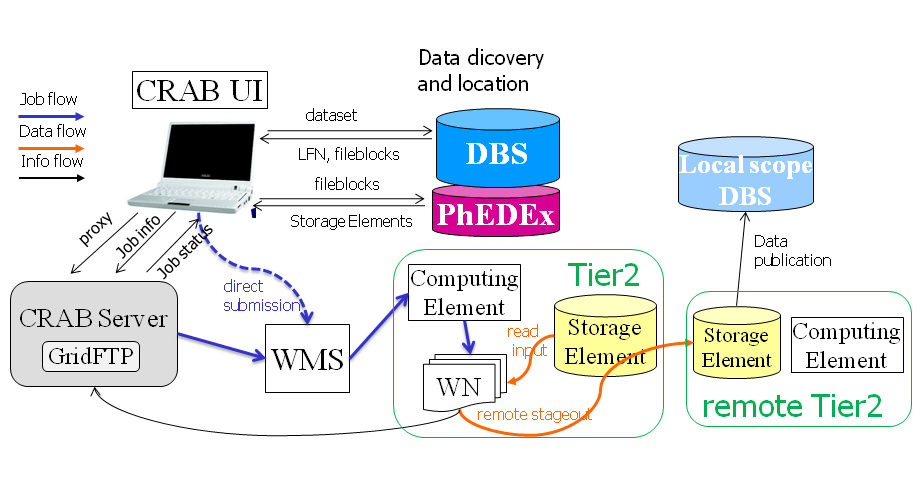
\includegraphics[width=0.70\textwidth]{figures/CRABWorkflow.png}
\caption{CRAB workflow. WMS can stand either for gLite WMS or glidein WMS.}
\label{fig:CRABWorkflow}
\end{figure}

\subsection{Monitoring}
\label{sec:3_3}
\subsubsection{Dashboard}

CMS Tier2's provide a large amount of resources in a fully distributed way,
spanning various
Grid organizations and middleware stacks
without any central place playing a reference role.
Each computing center has
different configuration, user community, policy, history and
constraints.
It was clear since the early days of CMS Analysis that
good monitoring tools are critical to the success of such
a highly distributed project, both to keep an overall
view of the usage and use patterns and to make it possible
to detect and address problems in an effective way,
using quantitative information to judge where to put
more effort and to evaluate the effectivness of solutions.
Good monitoring has allowed CMS to evolve tool development
and operational structure from vision and anedoctal driven
to a fact based approach.

Since the beginning a few main point drove the development of
those monitoring tools:
\begin{itemize}
\item no reliance on local site monitoring. It is not possible to ask
 all Tier2's to install some kind of CMS'owm ad hoc software, only the
 minimal grid service needed for grid interoperability can be expected.
\item a single entry point to the high level view of the usage from which
 it would be possible to drill down to detailed information at the single
  job level
\item  monitoring is not accounting: keep the system lean and
 flexible and do not worry if a small
 percentage of jobs is not properly reported
\item diagnose failures of users workflows so to
  take suggest corrective actions to developers and administrators, make
  enough proper information available so that plans and action are set
  based on quantitative facts and effectiveness of solutions can be metered
\item detect overall usage patterns to guide management into making
 choices and plans about how and were to steer user activities and
 how to plan for the future
\item do not try to define a priori the relevant metrics, usage, tools and
 hardware will always be changing and we expect the need to fight the
  problem of the month, different each month
\end{itemize}

That requires the capability to collect for most (ideally all) of the jobs
information like: execution and submission site, user, kind of activity,
accessed data, amount of I/O and CPU, efficiency of resource usage,
failure details (if any) and more and store it in some
place where data can be queried in various ways according to need.

Therefore job monitoring was built around the idea of instrumented
application: CMS jobs and tools send messages with a few relevant
parameters to a central collector, independently and in parallel to
whichever grid or monitoring system may exists, thus giving us
access to experiment specific information and giving independency
from execution sites. The price to pay is that only jobs that use the
instrumented submission framework can be monitored in this way.
This price turns out to be very small in CMS case, since almost
all user analysis jobs are submitted using the CRAB tool, which
inserts on user's behalf the needed reporting hooks.

The implementation of this idea comprises an optimised central
database running on Oraclo server, a set of information collectors
that feed data into it from various sources, a simple messaging
system to send information to the collector from the
CRAB tools running at submission location and job execution hosts,
and a few web pages providing access with different levels
of detail, aggregation and flexibility, customized to
typical use cases. This set of tools is called ''the CMS Dashboard''.

The Dashboard main collector is the one receiving messages from
CRAB user interface and CRAB wrapper used in running jobs, for thi
we used the already existing MonAlisa messaging system, which was
already proven to the needed scale. Other collectors add
information from gLite WMS and gLite LB hosts, adding in this way
information about the status of jobs while processed by the
middleware or local batch systems and allowing some limited
tracking of jobs submitted outside the CRAB tool.

The CMS dashboard collects information for both user jobs
(Analysis) and centrally controlled jobs (Production), providing
a comprehensive and uniform view of the CMS usage of computing
resources.

Three web interfaces are used to monitor and metere distributed analysis,
since those are different views of the same underlying database,
it is possible to cross link and navigate from one to another
providing both extreme flexibility and fast access to desired
informations

\subsection{History View}
The aim of this view is to present time history of relevant
metrics to get a view of overall patterns and trends.
%\figure{put a screenshot}
The list of viewable metrics is thus predefined, and
the interface uses aggregated tables in the DB to provide
efficient access to old information with (of course) a limited
amount of detail. Metrics can be viewed up to one year in the past
with granularity varying from fraction of a hour to a few days
according to the chosen time period. Data can be viewed divided
according e.g. to the used site(s), job type or job completion status.


\subsection{Task Monitoring for Analysis user}
Users usually submit many jobs in a single workflow, this
is called a Task in CRAB. Tasks usually have from a few hundred
to a thousand jobs each. A user will oftern submit one crab task
for each dataset used in a particular analysis, up to a few
tasks in one day. Task Monitoring for Analysis user was
developer as a user centric interface where the user is
initially presented the list of tasks he submitted in lasts
three days, both in tabular and graphical way.
%\figure{a screenshot}
The user can then expand one selected task to get
a graphical overall summary of execution/completion progress
and access details of each job.1
%\figure{another screenshot}

\subsection{Interactive Interface}
This view was the first to be developed, based on
vision more then experience with the tool, therefore
emphasis was put on flexibility. It is a job-centric view
where the entry point is the number of jobs submitted or
terminated in a chosen time period.
%\figure{a screenshot}
The interactive interface
allows then to drill down expanding the set of jobs by
various relevant properties (execution site, grid gateway,
submitter user, completions status, grid workload management host,
activity type, used dataset etc.), until all details stored in the DataBase
about a choosen (set of) job(s) can be accessed.
The interface reports success/failure values and fractions
according to grid/site/application problem and information
on used wall and cpu time of jobs.
The DataBase ahs been setup so to allow fast access for this
detailed information for the last two weeks, while queries
become more and more slow as time range expands. The idea is that
details are only needed to analyse current issues and for
long time view of trends the History View should be used.



\section{Operation of CMS Distributed Analysis}
\label{sec:4}
\subsection{Distributed Infrastructure}
\label{sec:4_1}

\subsubsection{ Grid services }
\label{sec:4_1_2}

The access to CMS resources is controlled by grid services provided by the WLCG project.

Users are authenticated via X.509 certificated issued by trusted Certificate Authorities (CA). Authorization is based on VOMS attribute certificates that certify the membership of users to the CMS Virtual Organization and possibly to CMS groups and the roles they have. VOMS servers are provided by the WLCG project.

Data are stored on systems exposing an SRM interface (Storage Elements). The specific implementation of the storage system is left to the sites (e.g. d-Cache, DPM, Castor, Storm, etc...). In CMS Tier-1s the storage systems also have a tape-based back-end to fulfil their custodial responsibilities, while at Tier-2s they are disk-based.

The access to computing resources (Compute Elements) is based on the Globus gatekeeper (on EGEE via its LCG-CE implementation) or on the ARC-CE on NorduGrid.

The CMS workload management system (CRAB and ProdAgent) may use, via the BossLite layer, several high level workload management tools provided by the different infrastructures. In particular the gLite WMS (by the EGEE projects), and the glide-in WMS (by OSG) are used to dispatch jobs to the different Compute Elements.

All computing and storage resources publish information on their characteristics and state to an Information System based on the BDII provided by WLCG. The information is used both for monitoring and for resource selection by the gLite-WMS.

The CMS data transfer system is implemented by Phedex that in turn depends on the gLite File Transfer System (FTS). WLCG maintains a number of FTS servers (at Tier-0 and Tier-1 sites) that define the transfer channels on which the transfers take place.

% FIXME Need to define where/how to use the following sentence
%CMS established a body to coordinate the operation of the facilities offering support to the experiment. The Facilities Operations team coordinates the operations at all sites (Tier-0, Tier-1s and Tier-2s) in close collaboration with the site managers and with the WLCG project.

\subsubsection{ SiteDB }
\label{sec:4_1_2}
%% From DanieleB
SiteDB is a catalogue of all CMS computing Tiers. It records the CMS resources at the site, the resources pledged for the future, and it keeps track of CMS personnel at each site, including the roles and duties they fulfull in the collaboration.
%Collaborators are automatically added to the SiteDB database on registering with the CMS Hypernews system. As well as providing the aforementioned information, SiteDB acts as a simple monitoring portal, bringing  in and providing links to content from PhEDEx, DBS, SAM tests, CMS Dashboard, GOCDB and GSTAT. The database also maintains a mapping between the different names a site can be known by, for instance the institute name (University of Bristol), its SAM/WLCG name (UKI-SOUTHGRID-BRIS-HEP), and the CMS name (T2_UK_SGrid_Bristol), as well as associations between sites (e.g. the parent T1 site for a T2)
CMS has designed and built SiteDB because CMS relies on close contact to the sites it uses. The distributed nature of CMS computing makes it very useful to track the people's responsbilities, and to contact them on the basis of their role. Some site roles are technical (for instance running PhEDEx) others are related to CMS computing policy (e.g. the site's Data Manager). 
%For users (both end users, and consumer of the info like the computing shifters) who have a problem with a site and may not know what the various roles and responsibilities are at a site, SiteDB provides this information. 
%In additions, SiteDB links to the CMS Savannah Computing Infrastructure portal, one of the tools CMS uses for internal  tracking of problems across the distributed infrastructure. In Savannah there is a group ('squad' in Savannah jargon) per site, dynamically maintained from the information in SiteDB via a set of cron-tabbed scripts.

\subsubsection{ Software Installation }
\label{sec:4_1_3}
Distributed analysis relies on the experiment software being pre-installed on the remote
sites for each release and removed when declared obsolete. 
The installation procedure is controlled centrally via high priority Grid jobs, which install the software on dedicated shared areas on the Compute Elements and also publish the versions available on the information system.

\subsection{Operational readiness}
\label{sec:4_2}
\subsubsection{ Site Readiness }
\label{sec:4_2_1} 
%systematically test each site and improve the availability of the Tier-1s and Tier-2 sites
%\emph{USE THE COMMISSIONING PAPER AT CHEP09 CR2009-089}
%\emph{USE site commissioning section in INTEGRATION PAPER AT CHEP09 CR2009-087}
The operation of the CMS distributed infrastructure requires a stable and reliable behaviour of the sites. CMS has established a procedure now routinely operated by the Facilities Operations team to extensively test all relevant aspects of sites supporting CMS, such as the ability to efficiently use their network to transfer data, the functionality of all the site services relevant for CMS and the capability to sustain the various CMS computing workflows at the required scale.

The procedure to evaluate the commissioning status of a site relies on several sources of information. Every day the following quantities are monitored: the CMS Site Availability Monitoring (SAM) tests, running on Grid site resources to check their basic functionality and the local CMS software and configuration; the success rate of the Job Robot, a load generator simulating user data analysis; the number and the quality of the data transfer links used in production by the site; the downtimes scheduled by the site. If any of the metrics based on the above information is not satisfied the site is declared in error state. A site is allowed to be in error state not more than two days over the last week, then it is declared "not ready". To recover from a "not ready state" the site needs to be ok for at least two consecutive days. In this way temporary glitches are allowed if recovered promptly.


\subsubsection{ Data transfer links }
\label{sec:4_2_2}
%% From DanieleB
An ad-hoc task force (Debugging Data Transfers,DDT)\cite{RefDDT} was created to coordinate the debugging of data transfer links, in order to commission most crucial transfer routes among CMS Tiers by designing and enforcing a clear procedure to debug problematic links. The DDT procedures are now part of the commissioned links overview.
\emph{USE DDT PAPER AT CHEP09 CR2009-093}


\subsection{Analysis Organization at CMS Sites}
\label{sec:4_3}
\subsubsection{ Organized Analysis Activities }
\label{sec:4_3_1}
In order to optimize the processing chain, CMS performs as many processing steps as possible in an organized way. 
Besides the re-processing %that is performed by the Data Operation team 
on the RAW data when improved reconstruction algorithms are available, a standard set of analysis passes is agreed with the physics groups and is performed promptly at the Tier-1 sites 
%by the CMS Data Operations team 
as the data arrive from the Tier-0 (or Tier-2 in case of simulated data). 
This step, known as skimming, performs data reduction both in terms of event size and number of events. 
The samples produced in this way are made available to the CMS physicists at the Tier-2s. % together with the AOD.

Normally only the team dealing with data processing operations %CMS Data Operations team 
has access to the Tier-1 resources but in some special cases 
some physicist may need access to large samples of RAW data. Examples of this kind of activity are the detector 
calibration or the Data Quality Monitor validation. Since the RAW data in general are not distributed to the Tier-2 sites, a special VOMS role has been created to grant access to the Tier-1s to those physicists. 

\subsubsection{ User and Physics Group Support }
\label{sec:4_3_2}
\paragraph{Physics group associations}
Physicist are organized in groups (Physics Groups, PG) each with its own internal organization. Each PG is associated with a few Tier-2 sites that support it by providing storage space and processing power. On the other hand each Tier-2 supports one or more PGs depending on its size.  Currently PGs may have access to all resources at Tier-2s but it is foreseen to exploit VOMS groups to optimize the support at sites.

\paragraph{Storage Hierarchy}
A nominal Tier-2 in 2008 had 200TB of disk-based storage. Making efficient use of the networking and ensuring the appropriate revision 
of a dataset is at a location with sufficient processing resources is a challenging data management exercise. The knowledge of the needs of many groups of people is aggregated in the group leaders and not in an automated software system. 

CMS has attempted to increase the number of people empowered to make data management decisions by
dividing the available storage into chunks. The 200TB of Tier-2 storage is divided into 4 logical
pieces. At the storage at the Tier-2s increases in 2009 and beyond the allocations to groups and
central space will grow.
\begin{itemize}
\item{} Local Group and User Space: This is roughly 30TB per group currently with an additional
1TB per user that is controlled and managed by the geographically local community.
\item{} Physics Group Space: 60-90TB of space is allocated to 2-3 physics analysis groups.
Representatives from the groups serve as data managers for the space and make subscription and deletion requests. The space for each group will increase with time as
datasets grow.
\item{} Centrally Controlled Space: 30TB (growing to 50TB in 2009) of space is identified at each Tier-2 under the control of CMS centrally. This is used to ensure complete copies of the
reconstruction datasets are available across the Tier-2s.
\item{} Simulation Staging and Temporary Space: 20TB is identified to stage simulation produced at the Tier-2s and other temporary files before they can either be merged or transferred to the permanent home.
\end{itemize}
%\emph{ central/user/group/production data }
%\emph{USE THE COMPUTING MODEL PAPER AT CHEP09 CR2009-084}
%Making efficient use of the networking and ensuring the appropriate revision of a dataset is at a location with sufficient processing resources is a challenging data management exercise. The knowledge of the needs of many
%groups of people is aggregated in the group leaders and not in an automated software system. CMS has attempted to increase the number of people empowered to make data management decisions by dividing the available storage into chunks. The 200TB of Tier-2 storage is divided into 4 logical pieces. At the storage at the Tier-2s increases in 2009 and beyond the allocations to groups and central space will grow.
%1. Local Group and User Space: This is roughly 30TB per group currently with an additional
%1TB per user that is controlled and managed by the geographically local community.
%2. Physics Group Space: 60-90TB of space is allocated to 2-3 physics analysis groups.
%Representatives from the groups serve as data managers for the space and make
%subscription and deletion requests. The space for each group will increase with time as datasets grow.
%3. Centrally Controlled Space: 30TB (growing to 50TB in 2009) of space is identified at each
%Tier-2 under the control of CMS centrally. This is used to ensure complete copies of the
%reconstruction datasets are available across the Tier-2s.
%4. Simulation Staging and Temporary Space: 20TB is identified to stage simulation produced at the Tier-2s and other temporary files before they can either be merged or transferred to the permanent home.
%CMS is in the process of training users and administrators to manage the storage at the Tier-2s to efficiently support analysis. Even in the current commissioning phase CMS has hundreds of active users and more than 5PB of disk space across the Tier-2s. We expect to utilize the space
%dynamically and take advantage of the wide area network links to update samples frequently.
%Shifting to this paradigm involves solving technical challenges as well as engaging a large community of users.
\paragraph{User support model}
User documentation is provided by a set of twiki pages composing the so called CMS Workbook. Documentation about the distributed environment and CRAB usage are available, as well as a troubleshouting guide.
Tutorials including hands-on session are periodically organized.
The day by day support is mainly performed via a mailing list (HyperNews) where
users reports the problems they are facing with. The reported problems ranges
 from problems with the infrastructure, site related issues to user's mistakes in tools configuration or real bug report that are feed back to developers.
The CMS Savannah Computing Infrastructure portal is used to report problems across the distributed infrastructure such as data access problems, problem on specific CMS software version at sites etc.

\section{Experience with CMS Distributed Analysis}
\label{sec:5}
\emph{intro about challanges and user experience....}

\subsection{Tests}
\label{sec:5_1}
During the Common Computing Readiness Challenge (CCRC08) in May 2008
various analysis exercises were performed to gain an overall understanding 
of the performance and readiness of the T2 sites for CMS data analysis.
Centrally organized job submissions were carried out both to understanding the site performance characteristics and to exercise closely the kind of workflows
expected by the physics groups.
\paragraph{Site performance measurement}
Different types of jobs, with increasing complexity, were used:
\begin{itemize}
\item long-running CPU intensive jobs with moderate I/O. This tests the basic submission and execution of an analysis job with no strenuous requirements on 
either submit rate, or I/O, or stageout. The goal here was to fill all batch slots available for the analysis at a given site without stressing the site.
\item long-running I/O intensive jobs provided some non negligible stress on 
the storage infrastructure at the sites.
\item short-running jobs O(10 min) with local stage out of O(10 MB) file as output. These jobs run for a short time, with many jobs finishing per hour, thus leading to a significant write request rate at large sites.
\end{itemize}
Up to 40 sites were involved across EGEE, OSG, and NorduGrid. More than 100,000 jobs succeeded throughout the challenge. The error rates were very mixed, ranging from less than 1\% at many sites to up to 50\% at a few sites due to
catastrophic storage failures. The failures were predominantly
due to storage problems at sites. In most but not all cases, those problems were detected and fixed by the site administrators within 24 hours. Ignoring the storage failures, the success rate in this exercise was found to be better than 99\%. Overall success rate including the storage issues, ranged between 92-99\% for these exercises.

\paragraph{Simualtion of physics group workflows}
An exercise to mimic realistic physics group activities running
on list of associated Tier2s was setup. 
%association of a list of T2s to each fake physics group
The CRAB server was used to submit realistic physics group tasks: 
analysis-like jobs reading a dataset at all sites and running for 
about 4 hours with remote stageout of a O(20 MB) output file to a subset of T2
sites. This simulates the computing model where each user has space at a T2 while the datasets are generally distributed throughout the world.
More than 100,000 jobs on about 30 sites were submitted in two weeks and 
the CRAB Server provided the needed functionality for job submission and 
tracking. %It is worth noting that the aim of this challenge was to test 
%the readiness of sites, by filling their resources, rather than a scale test of the CRAB Server.
Most failures were problems accessing the input data, from 0.1\%-10\% up to 50\% for pathological cases, and remote stageout issues were due to old Grid clients affecting from 100\% to few \% per site. These stageout issues were
promptly fixed by the site administrators. 
%Grid aborted jobswere usually reported via Global Grid User Support (GGUS)
%[] web with fast feedback from the sites. 
During the second week, sites with efficiency above 90\% significantly increased, as shown in Figure~\ref{fig:CCRC08SiteEff}.
%% mention the chaotic pahse?
\paragraph{Chaotic job submissions}
People from T2 sites were encouraged to submit jobs to other T2 sites, for mimicking a chaotic job submission pattern. This activity was clearly visible in the CMS Dashboard, showing lots of user activities at several sites. Figure~\ref{fig:CCRC08Chaotic} summarizes the number of active users per site, including T1s, T2s, T3s and opportunistic usage. Around 60 sites participated on these tests.

The CCRC08 analysis challenge drove the level of activity and participation at Tier2s to an unprecedented scale in CMS.

\begin{figure}
\centering
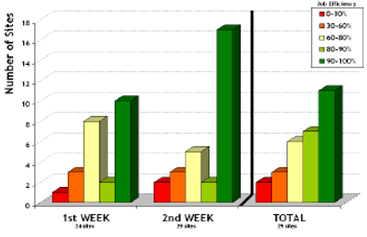
\includegraphics[width=0.55\textwidth]{figures/CCRC08SiteEff.png}
\caption{Distribution of the job efficiency by site, when simulating physics
groups workflows on CCRC’08}
\label{fig:CCRC08SiteEff}
\end{figure}
\begin{figure}
\centering
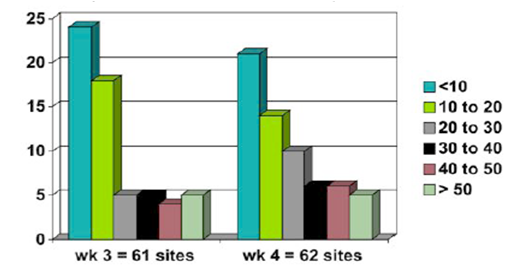
\includegraphics[width=0.55\textwidth]{figures/CCRC08Chaotic.png}
\caption{Chaotic phase}
\label{fig:CCRC08Chaotic}
\end{figure}

%% Scale test of CRAB server
\paragraph{CRAB Analysis server stress test} 
In order to test the CRAB server scalability and reliability up to
the expected CMS operational rates a dedicated test environment was
set up in October 2008. The Storage Element, based on GridFTP, 
that CRAB server relies on was installed on a different machine with 
respect to the machine hosting the CRAB Server components. The aim was 
to decouple the load
due the shipping of input/output sandboxes and the core workflow
management. The machine hosting the Storage Element and the CRAB
server were both 4 CPU 2000 MHz Dual Core AMD Opterons with 4 GB
RAM. The test was performed in the gLite context using two dedicated
gLite WMS. Monitoring information was collected from various sources
like the CRAB Server database tracking the job flow and the CPU usage
of its components, as well as from underlying services like MySQL and
GridFTP server and gLite WMS monitoring~\cite{wmsMon}. The kind of
jobs submitted were very short jobs running for less than a few
minutes, not reading a dataset and without stage-out. This choice was
made to provide an harsher environment for job handling due to higher
rate of finished jobs and to limit the resource usage at sites.

%\begin{itemize}
%\item{   Single user phase}
%
%A single user performed a controlled job submission pattern: peaks of
%1000-2000 jobs every 5 hours superimposed on a constant rate of
%500-600 jobs every 20 minutes. Almost 200,000 jobs were submitted to
%more than 50 sites with a rate above 40,000 jobs/day, as shown in
%Figure \ref{fig:stresssingle}. The CRAB Server was able to cope with that
%rate with no indication of reaching a breaking point. No significant
%backlogs were accumulated. The main contributors to the load of the
%system were the MySQL and GridFTP usage, using about 2 and 1.5 CPUs
%\begin{figure}
%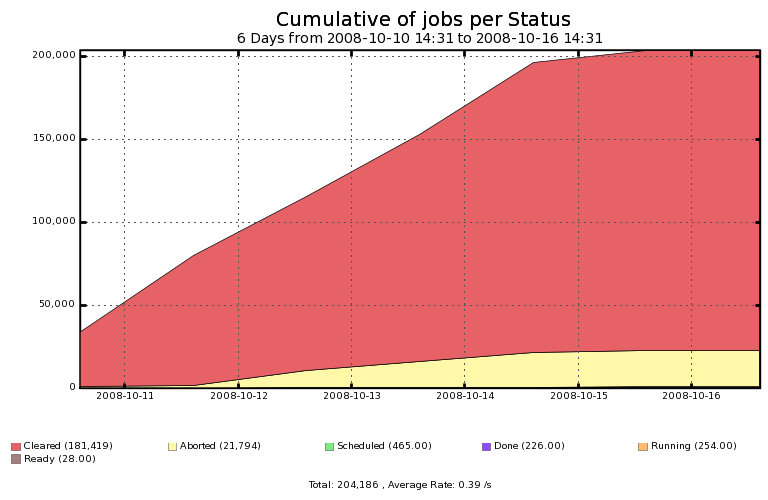
\includegraphics[width=0.55\textwidth]{figures/SingleUserJobStatus.png}
%\caption{Cumulative distribution of jobs submitted to CRAB Server
%  during the single user test phase. Aborted jobs were Grid related
%  problems at some sites. }
%\label{fig:stresssingle}
%\end{figure}
%
%\item{    Multi user environment phase}

Controlled submissions from different user certificates, thus 
emulating the CRAB Server usage in a multi-users environment, were performed.
%The need to further stress the multi-user environment arises
%from its higher complexity. Single threads of the very same component
%may be handling different user's jobs, requiring different
%certificates. Any interaction among them may cause failures, stopping
%the component work and causing a backlog.
Different submission patterns were adopted by the 12 users
involved. For example a user submitting 100 jobs every 15 minutes,
another 500 jobs every 20 minutes, another 2000 jobs every 6 hours
etc. plus a couple of users submitting randomly at their will.  No
CRAB Server misbehaviour was identified due to the multi-user
environment. %With respect to the single-user test 
Jobs were submitted to more than 50 sites with a rate above 50,000 jobs/day.
This helped identify some limitations in the communication between 
JobTracking and GetOutput components that caused a backlog of jobs without output retrieved. This effect is more evident for homogeneous very short
jobs, as those used in the test, that have a higher finishing rate
than real user's jobs which tend to finish at different times. None
the less, the backlog was absorbed in a few hours. This issue was
taken into account in the development cycle and the code was
optimized.  About 120,000 jobs were successfully handled in 48 hours,
as shown in Figure \ref{fig:stressmulti}.  The CPU load due to MySQL
proved to be stable regardless of the database size increase with more
jobs in the system. Overall the breakdown of CPU load usage is 2~CPUs
for MySQL, about 1.5~CPUs for GridFTP and about 1~CPU for all the CRAB
Server components, thus outlining the need of at least a 4~CPU
machine.  The load due to GridFTP is such that it's not compulsory to
have the GridFTP server decoupled from the machine hosting the CRAB
Server components.

Currently the whole CMS analysis is made of 30,000 jobs/day and the
CMS Computing model target is around 100,000-200,000 jobs/day. Some
CRAB Server instances deployed at different sites to serve physic's
group activities and regional community, as foreseen, can cope with
analysis needs.
%\end{itemize}
\begin{figure}
\centering
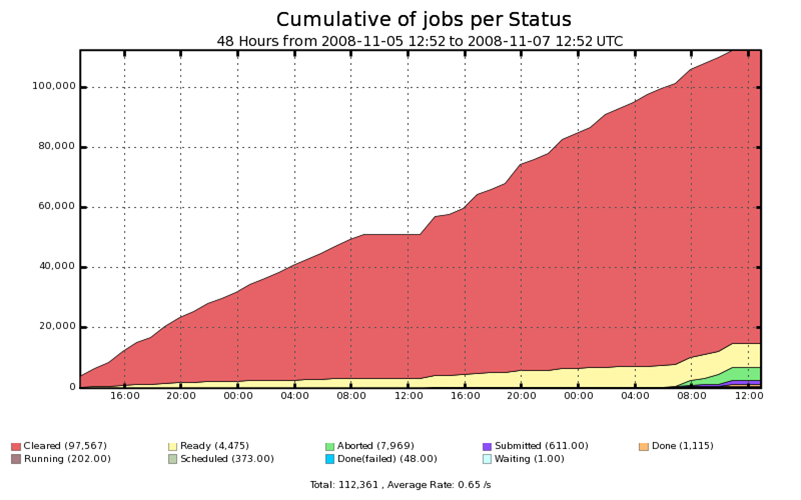
\includegraphics[width=0.55\textwidth]{figures/MultiUserJobStatus.png}
\caption{Cumulative distribution of jobs submitted to CRAB Server
  during the multi-user test phase. }
\label{fig:stressmulti}
\end{figure}



\subsection{Sustained Analysis}
\label{sec:5_2}

Distributed analysis is regularly performed by CMS users for MonteCarlo based analysis
and analysis of cosmic data collected in detector commissioning activities.


\emph{Look at metrics/content of PADA ASTF CHEP09 PAPER CR2009-088}

During last year about 11 million analysis jobs were submitted.  Peaks
of more than 100,000 jobs per day have been reached, with an average
of 30,000 jobs per day, as shown in Figure~\ref{fig:jobs}.
The distribution of jobs at Tier2s over the year is shown in Figure~\ref{fig:AnalysisJobHistoryMarch0809}. Current analysis activities has spontaneously surpassed, in term of number of jobs and number of sites, the scale reached in CCRC08 dedicated tests. 

\begin{figure}
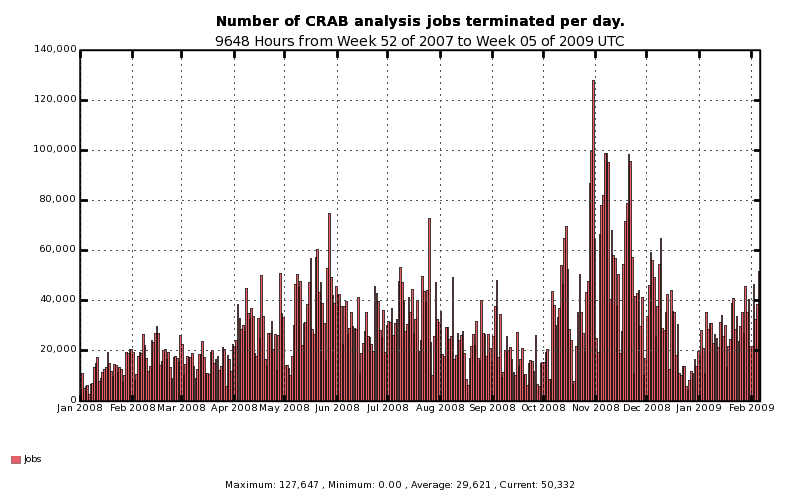
\includegraphics[width=3.5in]{figures/crabjobsdaily.png}
\caption{Number of daily jobs terminated in 2008. }
\label{fig:jobs}
\end{figure}
\begin{figure}
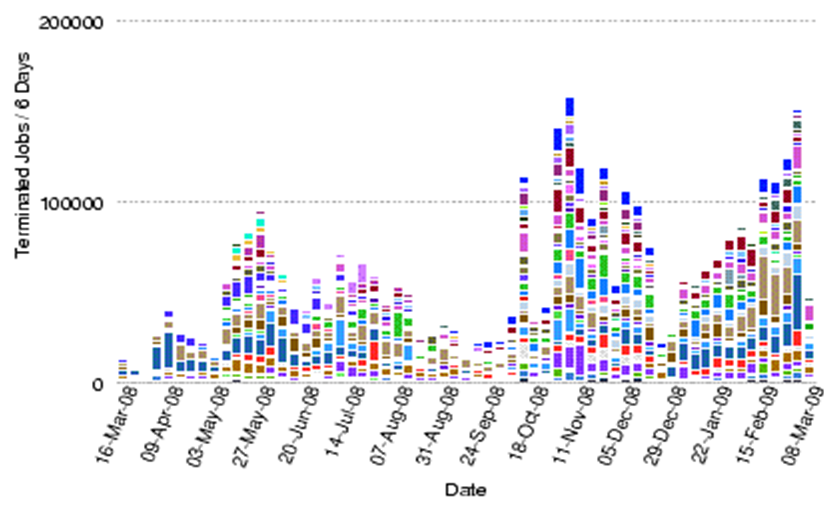
\includegraphics[width=0.7\textwidth]{figures/AnalysisJobHistoryMarch0809.png}
\caption{Number of analysis jobs by Tier2s during last year from CMS dashboard. Each color refers to a site. }
\label{fig:AnalysisJobHistoryMarch0809}
\end{figure}

\begin{figure}
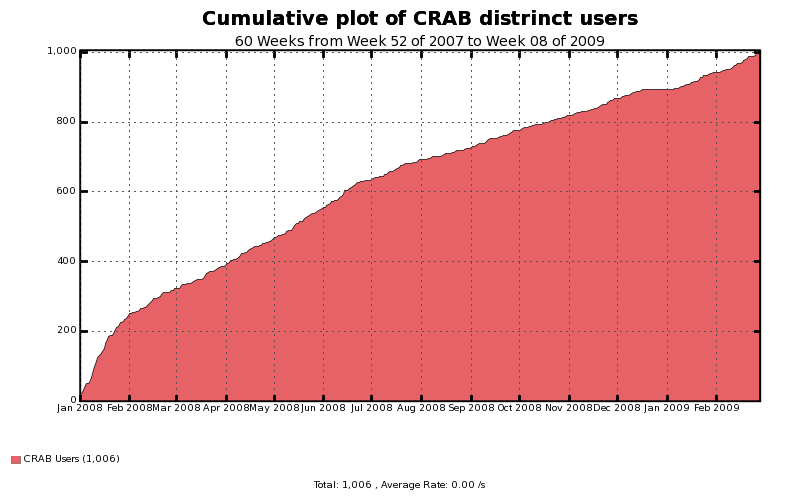
\includegraphics[width=3.5in]{figures/UserInteg.png}
\caption{Cumulative number of distinct CRAB users starting from 2008. }
\label{fig:intuser}
\end{figure}
\begin{figure}
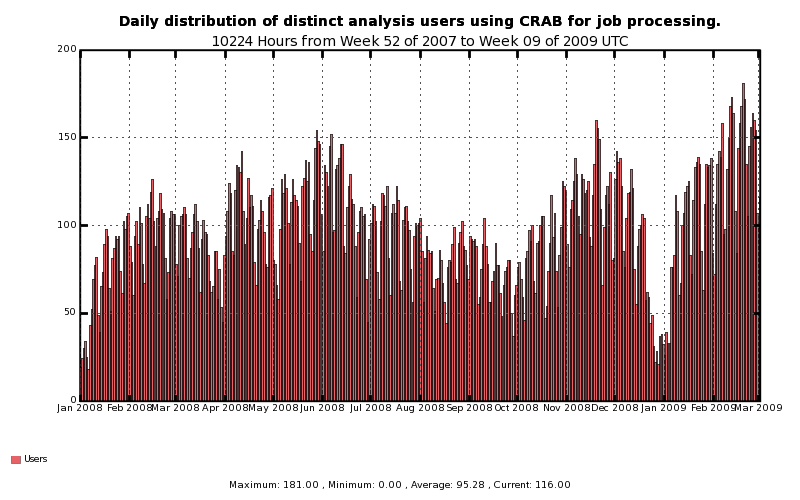
\includegraphics[width=3.5in]{figures/crabusersdaily.png}
\caption{Number of CRAB daily users in the 2008. }
\label{fig:distusers}
\end{figure}

Since 2008 the number of distinct CRAB users has grown to more than 1000, almost 30\% of the whole CMS
community, as shown in Figure~\ref{fig:intuser}. About 100 users per day use CRAB to submit their analysis jobs, 
as shown in Figure~\ref{fig:distusers}.


Analysis job efficiency is summaried in Fig.~\ref{fig:AnalysisJobEffMay08March09}. Most of the failures faced by the users are due to user application errors, remote stageout issues and errors reading data at the site. Application failures are expected, since analysis jobs run user code which may not have been
thoroughly tested.  Failures in stage out of the data output files to
remote storage can be due to users misconfiguring the remote
destination to use or to transfer problems. \emph{mention the foreseen approach for stageout}
Failures accessing data at the site mainly expose problems with the storage at the site or
inconsistencies between the data catalogue and what has been deleted at the site.  
A few percent of failures are due to jobs aborted by the Grid, however these are often due to site problems or jobs that spend
too much time on the worker node and are killed by the local batch system, appearing as aborted by the Grid.

% From Jan09 to May09:
% overall analysis job efficiency 62%
% breakdown of failures:
% - Grid failures
%   8% Grid Aborted jobs
% - Application errors:
%   35% remote stageout
%   22% CMSSW error (8001 , 8009) --> I suspect that some of the 8001
%                                      are due to error reading input files
%   13% error reading files at site (8020)
%    6.8% error 50115
\begin{figure}
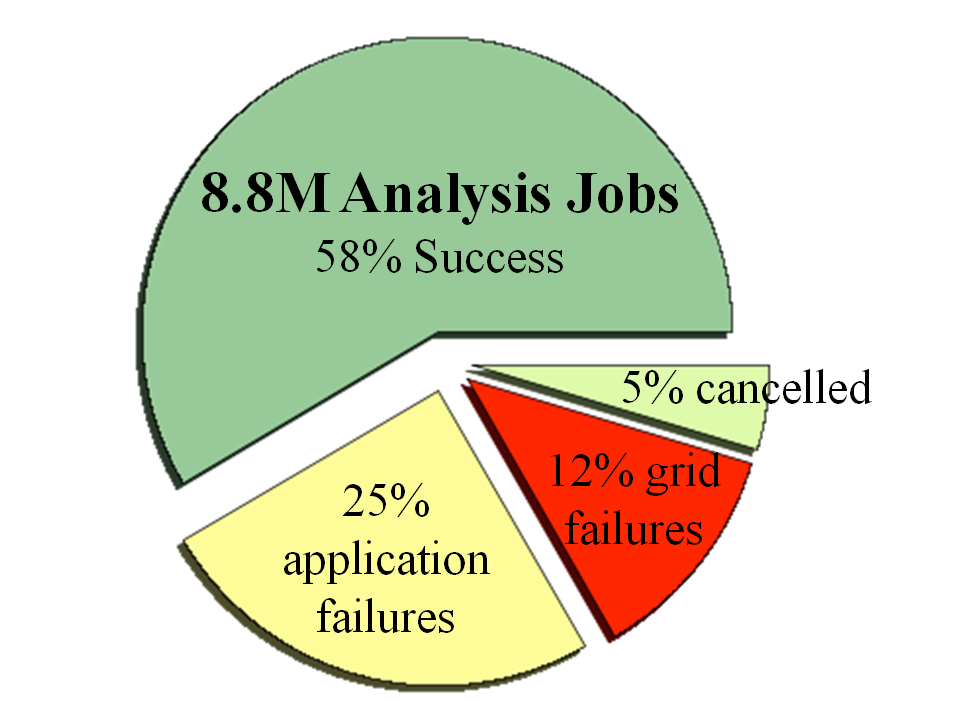
\includegraphics[width=0.5\textwidth]{figures/AnalysisJobEffMay08March09.png}
\caption{Analysis job efficiency from May 2008 to March 2009. \emph{If time and dashboard permits redo the py for one full year} }
\label{fig:AnalysisJobEffMay08March09}
\end{figure}

About 78\% of the CMS analysis jobs were submitted using gLite WMS.  Since the gLite architecture is such that the system scales linearly with the number of gLite WMSs used, analysis jobs are balanced currently over 7
WMS. The rest of the analysis jobs are submitted using Condor-G.

CRAB Analysis Server instances have been deployed in several countries (CERN, Italy, France). A couple of them are open to worldwide distributed CMS users. Other instances are being used by local communities or specific physics group.
For example the number of users using one server is shown in Fig.~\ref{fig:CSusers}.

\begin{figure}
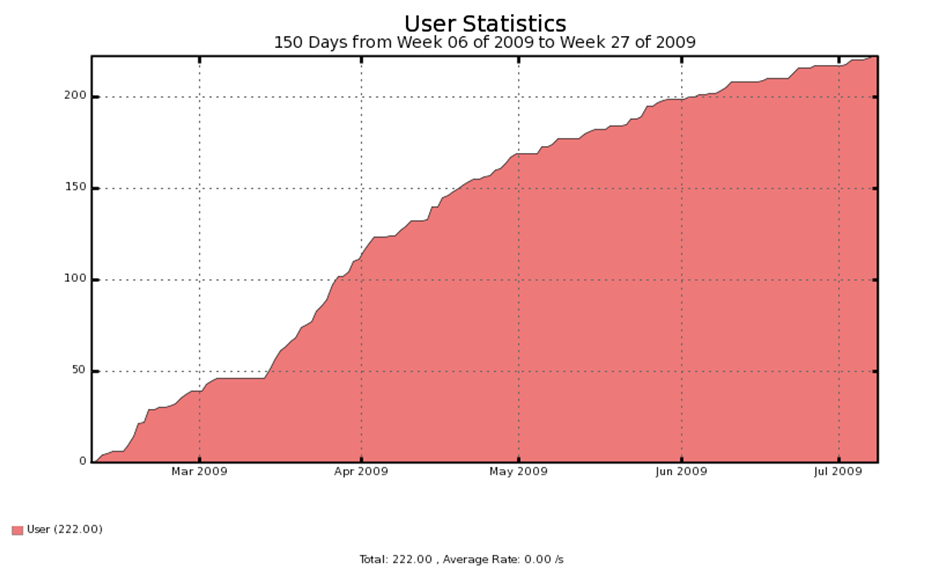
\includegraphics[width=0.5\textwidth]{figures/CSusersLast5months.png}
\caption{Number of distinct users using a CRAB server instance during last 5 months}
\label{fig:CSusers}
\end{figure}
In preparation for the LHC collision data taking real cosmic data are collected. 
\emph{briefly describe the CRAFT analysis exercise at T2s: 
\begin{itemize}
\item a set of paper being prepare assessing the detector performance plus some physics measurement
\item data distribution mainly at Muon Tier2s, but also at other sites for most popular skims
\item number of users Fig.~\ref{fig:CRAFTusers} and jobs Fig.~\ref{fig:CRAFTjobs} in CRAFT ( 2/3 of jobs at Tier2s and 1/3 at CAF)
\end{itemize}
}
\begin{figure}
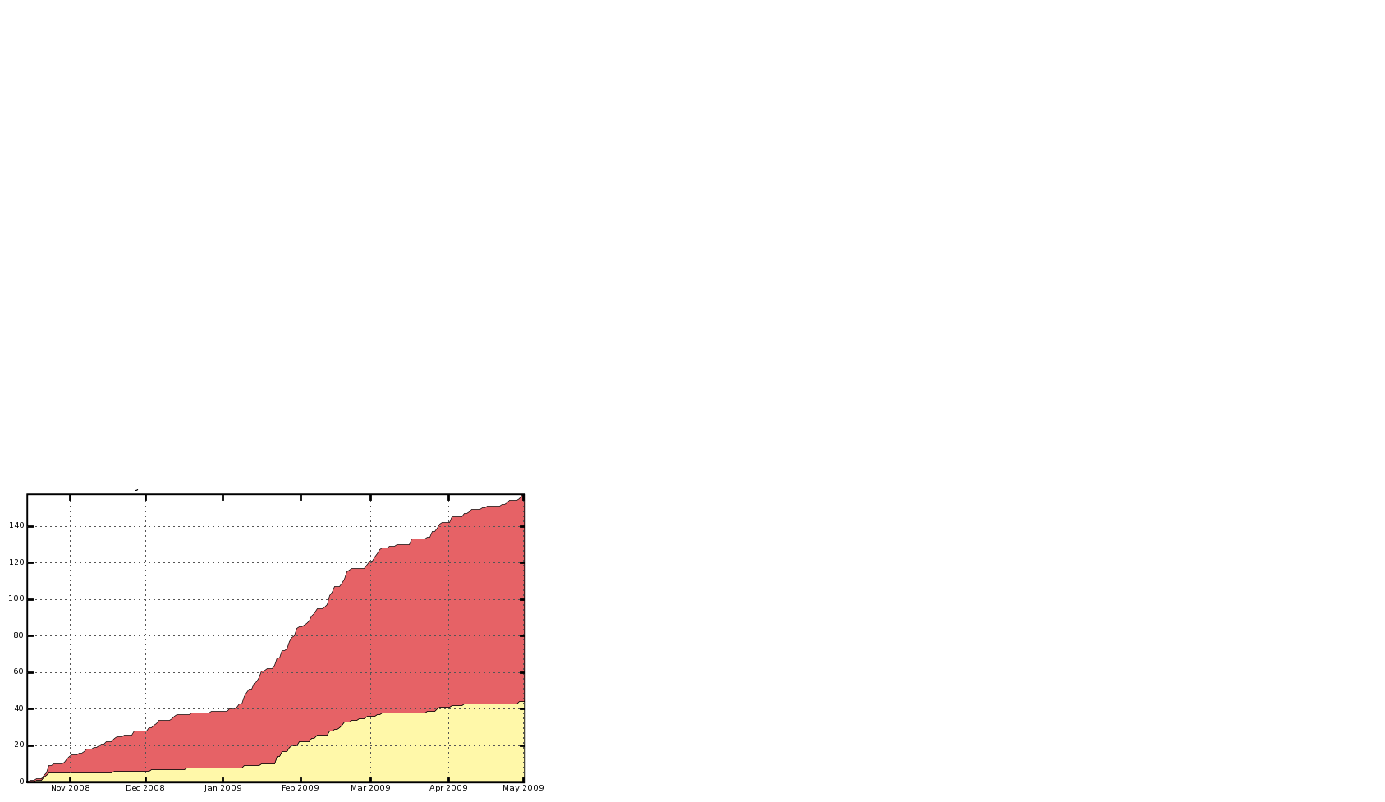
\includegraphics[width=0.5\textwidth]{figures/CRAFTusers.pdf}
\caption{Number of users analyzing CRAFT data using the CAF (light yellow) or the Tier2s(red).}
\label{fig:CRAFTusers}
\end{figure}
\begin{figure}
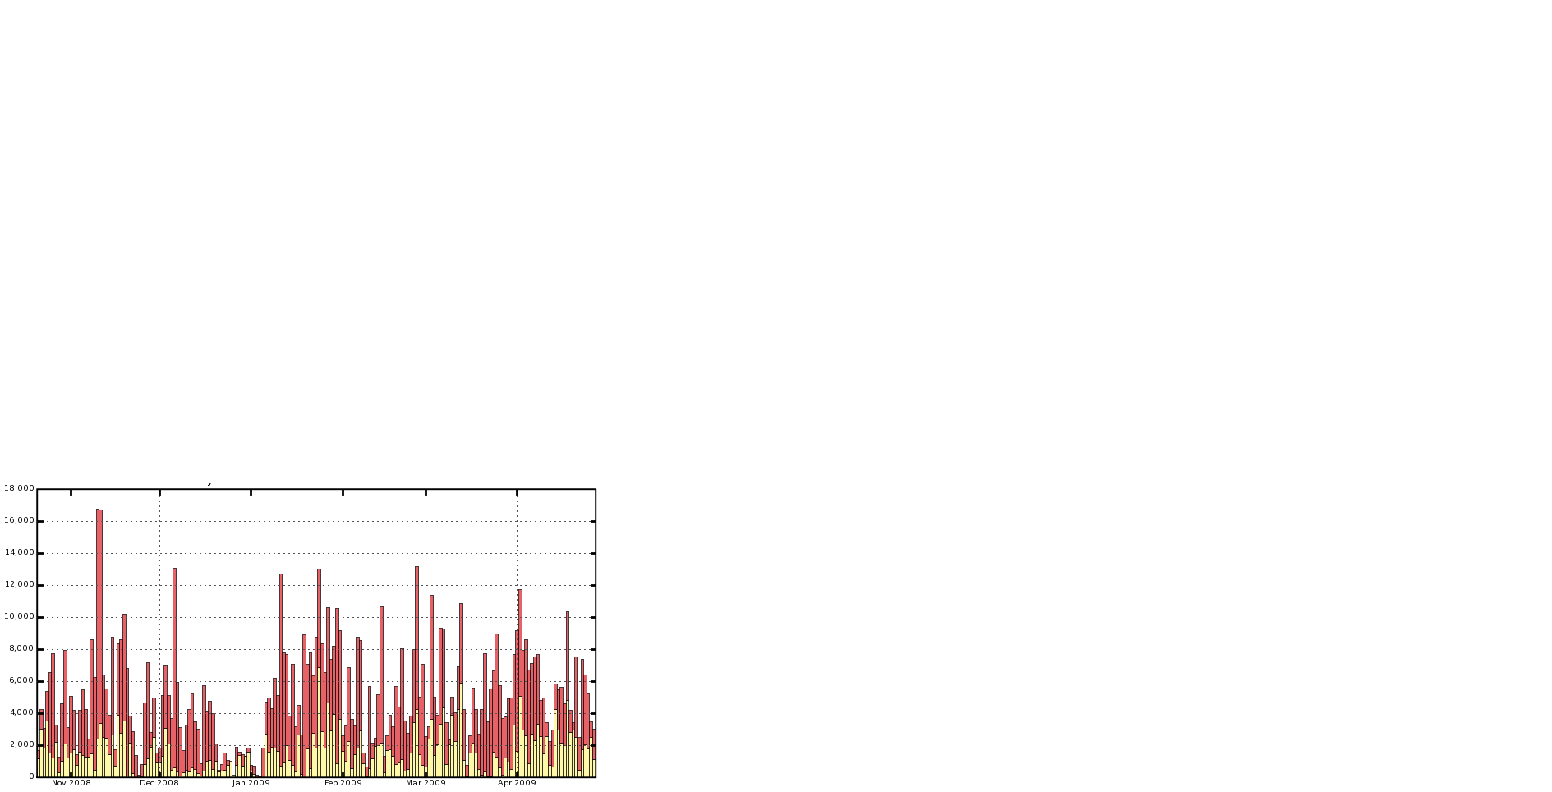
\includegraphics[width=0.5\textwidth]{figures/CRAFTjobs.pdf}
\caption{Number of jobs analyzing CRAFT data using the CAF (light yellow) or the Tier2s(red).}
\label{fig:CRAFTjobs}
\end{figure}



\section{Conclusions}
\label{sec:6}

% For one-column wide figures use
%\begin{figure}
%% Use the relevant command to insert your figure file.
%% For example, with the graphicx package use
%  \includegraphics{cations, both on the client-side and on the
%% figure caption is below the figure
%\caption{Please write your figure caption here}
%\label{fig:1}       % Give a unique label
%\end{figure}
%


%% For tables use
%\begin{table}
% table caption is above the table
%\caption{Please write your table caption here}
%\label{tab:1}       % Give a unique label
% For LaTeX tables use
%\begin{tabular}{lll}
%\hline\noalign{\smallskip}
%first & second & third  \\
%\noalign{\smallskip}\hline\noalign{\smallskip}
%number & number & number \\
%number & number & number \\
%\noalign{\smallskip}\hline
%\end{tabular}
%\end{table}

%\begin{acknowledgements}
%If you'd like to thank anyone, place your comments here
%and remove the percent signs.
%\end{acknowledgements}

% BibTeX users please use one of
%\bibliographystyle{spbasic}      % basic style, author-year citations
%\bibliographystyle{spmpsci}      % mathematics and physical sciences
%\bibliographystyle{spphys}       % APS-like style for physics
%\bibliography{}   % name your BibTeX data base

% Non-BibTeX users please use
\begin{thebibliography}{}
%
% and use \bibitem to create references. Consult the Instructions
% for authors for reference list style.
%
% Format for Journal Reference
\bibitem{RefCMS}
CMS Collaboration R. Adolphi et al., The CMS experiment at the CERN LHC, JINST, 0803, S08004 (2008)
%
\bibitem{RefCM}
CMS Collaboration, Computing Model TDR....
%
\bibitem{RefDBS}
A. Afaq et al., The CMS dataset bookkeeping service, J.Phys.Conf.Ser, 119, 072001 (2008)
%
\bibitem{RefPhEDEx}
L. Tuura et al., Scaling CMS data transfer system for LHC start-up, J.Phys.Conf.Ser, 119, 072030 (2008)
%
\bibitem{RefPA}
FIND A REFERENCE
%
\bibitem{RefCRAB}
D. Spiga et al., The CMS Remote Analysis Builder CRAB, 14th Int. Conf. on High Performance Computing ISBN/ISSN: 978-3-540-77219-4 , 4873, 580-586 (2007)\\
G. Codispoti et al., CRAB: a CMS Application for Distributed Analysis, to be published in TNS...
%
\bibitem{RefWLCG}
LCG Computing Grid Technical Design Report, LCG-TDR-001 CERN/LHCC 2005-024 (2005)
%
\bibitem{RefBOSSLite}
G. Codispoti et al., Use of the gLite-WMS in CMS for production and analysis, Proceedings of International Conference On Computing In High Energy Physics And Nuclear Physics (2009). \emph{IS IT POSSIBLE TO REFERNCE NOT YET PUBLISHED CHEP09 PAPER?}
%
\bibitem{RefgLiteWMS} P. Andreetto et al., The gLite Workload Management System, J.Phys.Conf.Ser, 119, 062007 (2008)
%
\bibitem{RefOSG} R. Pordes et al, The Open Science Grid, J.Phys.Conf.Ser, 78, 012057 (2007)
\bibitem{Refglidein} ADD A REFERENCE
%
\bibitem{RefARC} M.Ellertet al., Advanced Resource Connector middleware
  for lightweight computational Grids, Future Generation Computer Systems, 23, 219-240 (2007)
%
\bibitem{RefDDT} N. Magini et al., The CMS Data Transfer Test Environment in Preparation for LHC Data Taking, Proceedings of NSS-IEEE, Dresden (2008)  \emph{ARE THERE MORE DETAILED INFO ABOUT THIS RERENCE?}
%% Format for books
%\bibitem{RefB}
%Author, Book title, page numbers. Publisher, place (year)
\end{thebibliography}

\end{document}
% end of file template.tex

